\subsection{Rediseño del 'Arbol de An'alisis}

Para solucionar las limitaciones presentadas nos propusimos rediseñar el 'arbol de an'alisis.
El primer cambio que realizamos es la implementaci'on de \emph{heterogeneidad completa}.
Para lograr esto permitimos que también los secuentes sean heterogéneos, es decir, que puedan contener f'ormulas escritas en distintos lenguajes. De esta manera se consigue realizar las demostraciones con mayor flexibilidad y poder utilizar el lenguaje m'as apropiado para describir la propiedad que cada f'ormula enuncia.

En el 'arbol de an'alisis este cambio se refleja en la visualizaci'on de los nodos (Fig. \ref{hetero_homo}). Los nodos con secuentes heterogéneos se marcan con una \textit{H} mientras los nodos homogéneos no.

\begin{figure}[]
	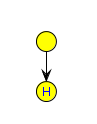
\includegraphics[width=50px]{img/hetero_homo.png}
	\centering
	\caption{El nodo con H contiene un secuente heterog'eneo. El otro nodo es homog'eneo.}
	\label{hetero_homo}
\end{figure}


\subsubsection{Ramas alternativas}

Para permitir documentar todas las acciones aplicadas as'i como la creaci'on de caminos de an'alisis alternativos introdujimos la noci'on de \textit{ramificaci'on alternativa}.
Las ramas alternativas representan la existencia de m'ultiples caminos en los que se subdivide el an'alisis para lograr un resultado. En la interfaz de usuario de Heterogenius este tipo de ramas se representa con lineas punteadas y se corresponde con un camino alternativo en una demostraci'on.

\begin{figure}[]
	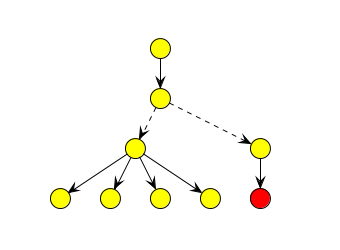
\includegraphics[width=180px]{img/ramas_alternativas_2.png}
	\centering
	\caption{La segunda rama alternativa presenta un contraejemplo. esto indica que existe un contraejemplo para el nodo del cual salen las ramas alternativas.}
        \label{alter1}
\end{figure}

Un nodo con hijos conectados por ramas alternativas se entiende que es demostrable si \textit{\textbf{alguna}} de las ramas es demostrable. Esto es diferente de la ramificaci'on normal (lineas continuas) que indica que la propiedad analizada y enunciada en el nodo padre puede ser demostrada si todos sus hijos llevan a una demostraci'on de las propiedades que cada uno enuncia.

Al aplicar una ramificaci'on alternativa a un nodo del 'arbol de an'alisis, el nodo es copiado y agregado como sus propios hijos, o sea el nodo sobre el que se aplica la acci'on, nodo $N$, pasa a tener dos hijos que son copias del nodo $N$. De 'esta forma se puede trabajar sobre los nuevos nodos $N$ como si fuera el original.
 
La principal ventaja de usar caminos alternativos es la de poder documentar todo el an'alisis que se realiz'o y las decisiones tomadas, incluso las decisiones que no llevaron al cumplimiento del objetivo. Por otro lado tambi'en nos permite experimentar con diferentes formas de probar lo mismo.
En las Fig.~\ref{alter1} y \ref{alter2} se muestran ejemplos de estos usos.

\begin{figure}[]
	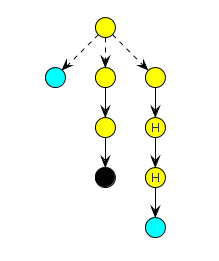
\includegraphics[width=100px]{img/ramas_alternativas.png}
	\centering
	\caption{Tres ramas alternativas: la primera y la 'ultima indican que no se encontr'o ning'un contraejemplo. La segunda rama muestra que se pudo demostrar que el secuente vale, por lo cu'al el secuente del nodo raiz tambi'en vale.}
        \label{alter2}
\end{figure}



\subsubsection{Nueva Clasificaci'on de Acciones}

Como se ha mencionado en la secci'on \ref{section:Heterogenius}, el elemento principal del proceso de demostración en Heterogenius es el 'arbol de an'alisis. El 'arbol soporta ciertas acciones cuya clasificaci'on se detalla anteriormente.

Si bien esta clasificaci'on serv'ia en la versi'on anterior, debi'o ser modificada para adaptarse a la nueva funcionalidad incluida durante el desarrollo de este trabajo y permitir una mayor flexibilidad a la hora de agregar otras herramientas en el futuro.
La nueva clasificaci'on propuesta se muestra a continuaci'on.

\begin{description}
\item[\textbf{Acciones de c'alculo de secuentes}:] esta categor'ia es ls misma que en la versi'on anterior. Comprende las acciones que permiten avanzar en el an'alisis aplicando reglas del c'alculo de secuentes.

\item[\textbf{Acciones de herramientas estructurales}:] son acciones que trabajan directamente sobre la estructura del 'arbol de an'alisis. Los traductores-$\rho$ forman parte de 'este grupo, asi como las nuevas acciones introducidas: \textit{traducci'on-$\rho$ de f'ormulas} y \textit{proyecci'on de f'ormulas}.

\item[\textbf{Acciones de herramientas automáticas}:] este grupo representa a las acciones para las que se usan herramientas autom'aticas como lo son los demostradores autom'aticos de teoremas y los buscadores de contraejemplos.
\end{description}

Esta clasificaci'on se reflej'o en la arquitectura de Heterogenius y permitir'a guiar las futuras extensiones y funcionalidades adicionales que se deseen implementar.
